\documentclass[border=10pt]{standalone}

\usepackage{tikz}
\usepackage{tikzsymbols}
\usetikzlibrary{calc,patterns,shapes.geometric}

\def\centerarc[#1](#2)(#3:#4:#5){\draw[#1] ($(#2)+({#5*cos(#3)},{#5*sin(#3)})$) arc (#3:#4:#5);}

\begin{document}
	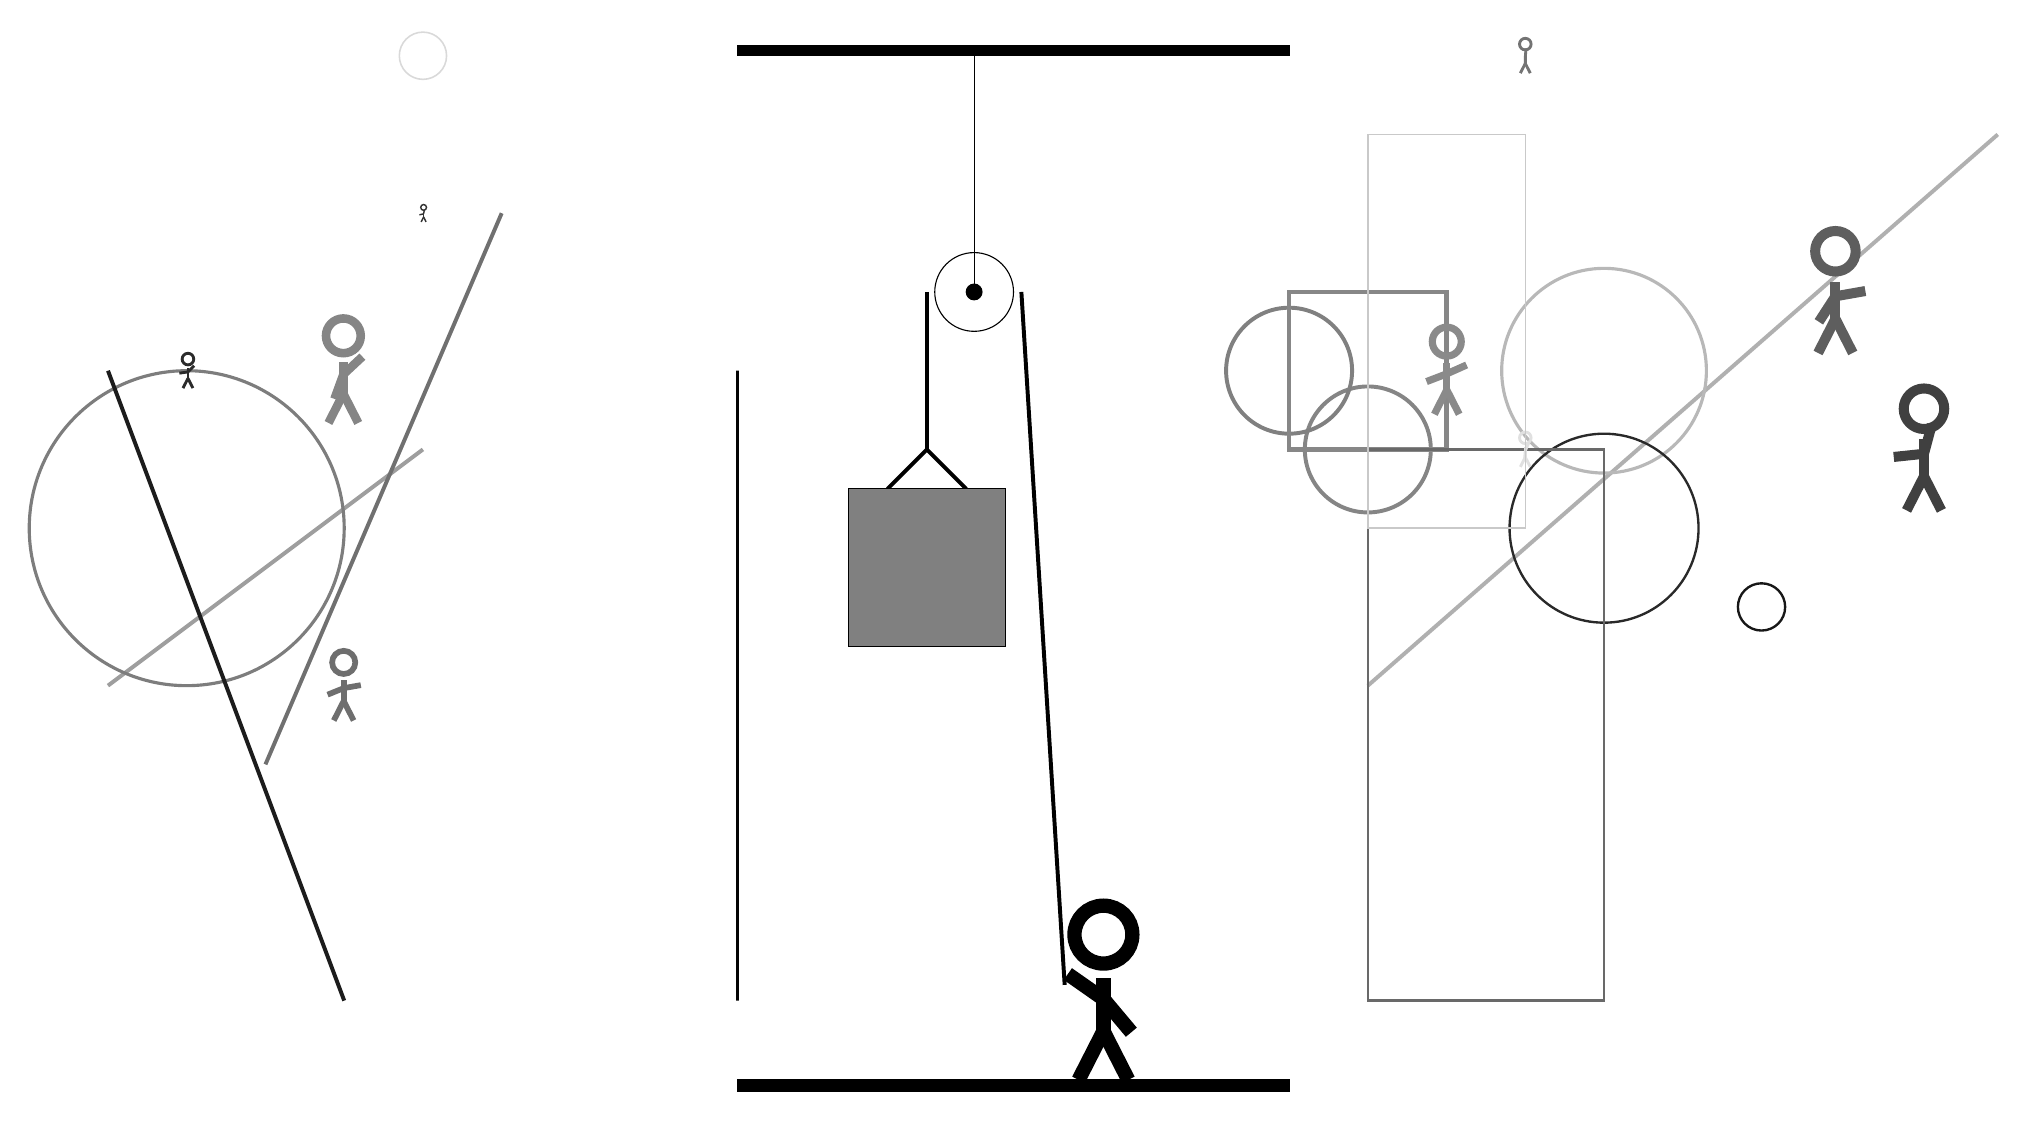
\begin{tikzpicture}
		%%%%% START %%%%%
		
		\draw[fill=black] (-2, 10) rectangle (5, 10.125);
		
		\draw (1, 7) circle (0.5);
		\draw[fill=black] (1, 7) circle (0.1);
		\draw (1, 10) -- (1, 7);
		
		\draw[line width=0.5mm] (-0.1, 4.5) -- (0.4, 5.0) -- (0.9, 4.5);
		\draw[fill=black!50] (-0.6, 4.5) rectangle (1.4, 2.5);
		
		\draw[line width=0.5mm] (0.4, 7) -- (0.4, 5.0);
		\centerarc[line width=0.5mm](1, 7)(0:180:0.6);
		\draw[line width=0.5mm](1.6, 7) -- (2.15, -1.8);
		
		\node at (2.6, -1.9) {\Strichmaxerl[10][-35][-50]};
		
		\draw[line width=0.5mm, color=black!31](6, 2) -- (14, 9);
		
		\draw[line width=0.5mm, color=black!38](-6, 5) -- (-10, 2);
		\node[line width=0.4mm, color=black!63] at (12, 7) {\Strichmaxerl[7][57][10]};
		\node[line width=0.5mm, color=black!57] at (-7, 2) {\Strichmaxerl[4][22][10]};
		
		\draw [line width=0.5mm, color=black!48](6, 5) circle (0.8);
		\draw [line width=0.2mm, color=black!15](-6, 10) circle (0.3);
		
		\draw [line width=0.5mm, color=black!50](5, 6) circle (0.8);
		
		\draw [line width=0.4mm, color=black!51](-9, 4) circle (2.0);
		\node[line width=0.5mm, color=black!83] at (-9, 6) {\Strichmaxerl[2][8][45]};
		\draw[line width=0.6mm, color=black!47] (7, 7) rectangle (5, 5);
		\draw[line width=0.4mm, color=black!99] (-2, -2) rectangle (-2, 6);
		\node[line width=0.3mm, color=black!48] at (-7, 6) {\Strichmaxerl[6][70][43]};
		\node[line width=0.6mm, color=black!46] at (7, 6) {\Strichmaxerl[5][21][24]};
		
		\node[line width=0.6mm, color=black!80] at (-6, 8) {\Strichmaxerl[1][13][80]};
		\node[line width=0.7mm, color=black!55] at (8, 10) {\Strichmaxerl[2][89][85]};
		\draw [line width=0.4mm, color=black!28](9, 6) circle (1.3);
		
		\draw [line width=0.3mm, color=black!84](9, 4) circle (1.2);
		
		\draw[line width=0.5mm, color=black!56](-5, 8) -- (-8, 1);
		\draw[line width=0.3mm, color=black!59] (6, -2) rectangle (9, 5);
		\node[line width=0.4mm, color=black!12] at (8, 5) {\Strichmaxerl[2][85][66]};
		\draw[line width=0.2mm, color=black!21] (6, 4) rectangle (8, 9);
		
		\draw[line width=0.2mm, color=black!96] (-4, 3) rectangle (-4, 3);
		\draw[line width=0.5mm, color=black!89](-7, -2) -- (-10, 6);
		\node[line width=0.6mm, color=black!75] at (13, 5) {\Strichmaxerl[7][6][75]};
		\draw [line width=0.3mm, color=black!91](11, 3) circle (0.3);
		
		
		\draw[fill=black] (-2, -3) rectangle (5, -3.15);
		
		%%%%% END %%%%%
	\end{tikzpicture}
\end{document}